%\RequirePackage{snapshot}
\documentclass{overturerepchap}
%**********************************************************
%
% Bibliography support
%
%**********************************************************
%\def\@reportno{YY--NN}		% default report no.
%\def\reportno#1{\gdef\@reportno{#1}}
\usepackage{capt-of}
\usepackage{multirow}
\usepackage{fancyhdr}
\usepackage{longtable}
\newcommand{\bthisbibliography}[1]{\chapter*{References}%
   \begin {list} {}%
     {\settowidth {\labelwidth} {[#1]XX}%
      \setlength {\leftmargin} {\labelwidth}%
      \addtolength{\leftmargin} {\labelsep}%
      \setlength {\parsep} {1ex}%
      \setlength {\itemsep} {2ex}%
     }
  }
\newcommand{\ethisbibliography}{\end{list}}
\newcommand{\refitem}[2]
  {\bibitem[#1]{#2}}

\newcommand{\back}{$\setminus$}
\newcommand{\RuleTarget}[1]{\hypertarget{rule:#1}{}}
\newcommand{\Ruledef}[2]
{
  \RuleTarget{#1}\Rule{#1}{#2}%
  }
\newcommand{\Ruleref}[1]{
  \hyperlink{rule:#1}{#1}}
\newcommand{\Lit}[1]{`{\tt #1}\Quote}
\newcommand{\Rule}[2]{
  \begin{quote}\begin{tabbing}
    #1\index{#1}\ \ \= = \ \ \= #2  ; %    Adds production rule to index

  \end{tabbing}\end{quote}
  }
%%%%%%%%%%%%%%%%%%%%%%%%%%%%%%%%%%%%%%%%%%%%%%%%%%%%%%%%%%%%%
%%% Model transformation rule box
%%%%%%%%%%%%%%%%%%%%%%%%%%%%%%%%%%%%%%%%%%%%%%%%%%%%%%%%%%%%%
\newcounter{formationRule}
\setcounter{formationRule}{0}
\newenvironment{formationRule}
%{\refstepcounter{formationRule}\vspace{10pt}\par\noindent
%Exercise \theformationRule
%\begin{itshape}\par\noindent\vspace{10pt}}%
%{\end{itshape}\vspace{10pt}\par}
{%
\refstepcounter{formationRule}
%increment
%\addtocounter{transformationRuleCounter}{1}%
%\ctf{}%
%\labelformat{formationRule}{\value{formationRule}}
\begin{center}%
\begin{tabular}{ | p{10cm} |}\hline%
\textbf{Transformation Rule \theformationRule}

}
{
\\
    \hline
    \end{tabular}
\end{center}

}
\newcommand{\kw}[1]{{\textbf\ttfamily #1}}
\newcommand{\SeqPt}[1]{\{\ #1\ \}}
\newcommand{\lfeed}{\\ \> \>}
\newcommand{\dsepl}{\ $|$\ }
\newcommand{\dsep}{\\ \> $|$ \>}
\newcommand{\Lop}[1]{`{\sf #1}\Quote}
\newcommand{\blankline}{\vspace{\baselineskip}}
\newcommand{\Brack}[1]{(\ #1\ )}
\newcommand{\nmk}{\footnotemark}
\newcommand{\ntext}[1]{\footnotetext{{\bf Note: } #1}}
\newlength{\kwlen}
\newcommand{\Keyw}[1]{\settowidth{\kwlen}{\tt #1}\makebox[\kwlen][l]{\sf
    #1}}
\newcommand{\keyw}[1]{{\sf #1}}
\newcommand{\id}[1]{{\tt #1}}
\newcommand{\metaiv}[1]{\begin{alltt}\input{#1}\end{alltt}}

\newcommand{\OptPt}[1]{[\ #1\ ]}
\newcommand{\MAP}[2]{\kw{map }#1\kw{ to }#2}
\newcommand{\INMAP}[2]{\kw{inmap }#1\kw{ to }#2}
\newcommand{\SEQ}[1]{\kw{seq of }#1}
\newcommand{\NSEQ}[1]{\kw{seq1 of }#1}
\newcommand{\SET}[1]{\kw{set of }#1}
\newcommand{\PROD}[2]{#1 * #2}
\newcommand{\TO}[2]{$#1 \To #2$}
\newcommand{\FUN}[2]{#1 \To #2}
\newcommand{\PUBLIC}{\ifthenelse{\boolean{VDMpp}}{public\mbox{}}{\mbox{}}}
\newcommand{\PRIVATE}{\ifthenelse{\boolean{VDMpp}}{private}{\mbox{}}}
\newcommand{\PROTECTED}{\ifthenelse{\boolean{VDMpp}}{protected}{\mbox{}}}

\pagestyle{fancy}
\fancyhead{}
\fancyhead[LO]{\leftmark}
\fancyhead[RE]{Overture VSCode Tool Support: User Guide}
\fancyhead[RO,LE]{\resizebox{0.05\textwidth}{!}{\includegraphics{overture}}}
\fancyfoot[C]{\thepage}

\usepackage{makeidx}

\usepackage{graphicx, color}

% definition of VDM++, JavaCC, JJTree, JTB, ANTLR and SableCC for listings
\newcommand{\NL}{\mbox{}\\ \vspace*{-5mm}}
\usepackage{listings}
\newcommand{\url}[1]{\texttt{#1}}
\usepackage{vdmsl-2e}
\usepackage{hyperref}

\usepackage{times}
\usepackage{color}
\include{customlangdef}
% define the layout for listings
\lstdefinestyle{tool}{basicstyle=\ttfamily,
                         frame=trBL,
			 showstringspaces=false,
			 frameround=ffff,
			 framexleftmargin=0mm,
			 framexrightmargin=0mm}
\lstdefinestyle{mystyle}{basicstyle=\footnotesize\ttfamily,
                         frame=trBL,
%                         numbers=left,
%			 gobble=0,
%			 basewidth=0.51em,
                         showstringspaces=false,
%			 linewidth=\textwidth,
			 frameround=fttt,
			 aboveskip=2mm,
			 belowskip=2mm,
			 framexleftmargin=0mm,
			 framexrightmargin=0mm}
%\lstdefinestyle{mystyle}{basicstyle=\sffamily\small,
%			 frame=tb,
%                         numbers=left,
%			 gobble=0,
%			 showstringspaces=false,
%			 linewidth=345pt,
%			 frameround=ffff,
%			 framexleftmargin=8mm,
%			 framexrightmargin=8mm,
%			 framextopmargin=1mm,
%			 framexbottommargin=1mm,
%			 aboveskip=7mm,
%			 belowskip=5mm,
%			 xleftmargin=10mm,}

\lstset{style=mystyle}
\lstset{language=VDM++}
%\lstset{alsolanguage=Java}
% The command below enables you to escape into normal LaTeX mode inside your
% VDM chunks by starting with a `^' character and ending with a `^'
\lstset{escapeinside=\^\^}

%This file has been converted to use LaTeX2e
%\documentstyle[overture]{article}
%
% any "\include{...}" statements go here
%
%\include{ifad}
%\include{graphics}
\usepackage{cite}
\usepackage{alltt}
%\usepackage{fancyhdr}
\renewcommand{\topfraction}{0.9}
\renewcommand{\textfraction}{0.05}
\renewcommand{\floatpagefraction}{0.9}
\makeindex

\begin{document}
\title{Overture VSCode Extension Support: User Guide \\{\large Version 0.0.1}}
\author{Tom Montout, Hugo Daniel Macedo, Jonas K. Rask, Peter Gorm Larsen\\
Aarhus University, Department of Engineering\\
Finlandsgade 22, DK-8000 \AA{}rhus C, Denmark\\[3mm]
Nick Battle\\
Fujitsu UK\\
Lovelace Road, Bracknell, \\
Berkshire. RG12 8SN, UK}

\date{August 2021}

\reportno{TR-007}

\maketitle


\textbf{Document history}

\begin{tabular}{|l|l|l|l|}\hline
Month   & Year & Version & Version of Overture\\ \hline
August & 2021 &         & 0.0.1 \\ \hline
\end{tabular}

\tableofcontents

\let\cleardoublepage\clearpage

\begin{abstract}
This document is the user manual for the Overture VSCode Extension supporting the Vienna Development Method
(VDM). It serves as a reference for anybody wishing to make use of
the tool with one of the VDM dialects (VDM-SL, VDM++ or VDM-RT). 
The different dialects are controlled by a VDM language Board that 
evaluates possible Requests for Modifications.
Overture tool support is built on top of the VSCode platform. The
objective of the Overture initiative is to create and support an open source
platform that can be used for both experimentation with new VDM dialects,
as well as new features for analysing VDM
models in different ways. The tool is entirely open source, so anybody
can join the development team and influence future
developments. The goal is to ensure that stable
versions of the tool suite can be used for large scale industrial
applications of VDM technology.
\end{abstract}

\chapter{Introduction}

The Vienna Development Method (VDM) is one of the longest established
model-oriented formal methods for the development of computer-based
systems and software
\cite{Bjorner&78,Jones90a,Fitzgerald&08c}. It consists of a
group of mathematically well-founded languages for expressing system
models during early design stages, before expensive implementation
commitments are made. The construction and analysis of a model using
VDM helps to identify areas of incompleteness or ambiguity in
informal system specifications, and provides some level of confidence
that a valid implementation will have key properties, especially those
of safety or security. VDM has a strong record of industrial
application, in many cases has been used
by practitioners who were not specialists in
the underlying formalism or logic
\cite{Larsen&96b,Clement&99,Kurita&09}. Experience with the method
suggests that the effort spend on formal modelling and analysis can
be recovered in reduced rework costs arising from design errors.

VDM models can be expressed in a Specification Language (VDM-SL) which
supports the description of data and functionality
\cite{ISOVDM96a,Fitzgerald&98b,Fitzgerald&09}. Data are defined by
means of types built using constructors that define structured data
and collections such as sets, sequences and mappings from basic values
such as Booleans and natural numbers. These types are very abstract,
allowing you to add any relevant constraints using data type
invariants. Functionality is defined in terms of operations over these
data types. Operations can be defined implicitly by preconditions and
postconditions that characterise their behavior, or explicitly by
means of specific algorithms. An extension of VDM-SL, called VDM++,
supports object-oriented structuring of models and permits direct
modelling of concurrency \cite{Fitzgerald&05}. A further extension
to VDM++, called VDM Real Time (VDM-RT\footnote{Formerly called VDM In a
Constrained Environment (VICE).}), includes support for discrete
time models \cite{Mukherjee&00,Verhoef&06b}. The VDM-RT dialect is also used inside 
the Crescendo tool\footnote{See \url{http://crescendotool.org/}.} supporting collaborative modelling and co-simulation \cite{Fitzgerald&14c}. All
three VDM dialects are supported by Overture.

Since VDM modelling languages have a formal mathematical semantics,
a wide range of ana\-ly\-ses can be performed on models, both to check
internal consistency and to confirm that models have emergent
properties. Analyses may be performed by inspection, static analysis,
testing or mathematical proof. To assist in this process, Overture
offers tool support for building models in collaboration with other
modelling tools, to execute and test models and to carry out different
forms of static analysis \cite{Larsen&13b}. It can be seen as an open
source version of the closed (but now freely available) tool called VDMTools
\cite{Elmstrom&94,Larsen01,Fitzgerald&08a}.

This guide explains how to use the Overture VDM VSCode Extension for developing models
for different VDM dialects. It starts with an explanation
of how to get hold of the software in
Chapter~\ref{sec:install}. This is followed in
Chapter~\ref{sec:vdmsupport} with an introduction to the VSCode
workspace terminology. Chapter~\ref{sec:projects} explains how
projects are managed in the Overture VSCode Extension. Chapter~\ref{sec:editVDM}
covers the features for creating and editing VDM models. This is
followed in Chapter~\ref{sec:debug} with an explanation of the
interpretation and debugging capabilities in Overture.
Chapter~\ref{sec:testcoverage} illustrates how test coverage
information can be gathered when models are interpreted.
Chapter~\ref{sec:prettyprint} shows how models with test
coverage information can be written as
\LaTeX\ and automatically converted to PDF format.
Chapters~\ref{sec:POmanagement} to \ref{sec:codegen} cover various
VDM specific features: Chapter~\ref{sec:POmanagement}
explains the notion of proof obligations and their support in
Overture; Chapter~\ref{sec:testing} explains
combinatorial testing and the automation support for that; Chapter~\ref{sec:codegen} explains
how it is possible automatically to generate executable code in programming languages such as Java for a subset of VDM models;
Appendix~\ref{app:templates} provides a list
of all the standard templates built into Overture.
Appendixes~\ref{app:internalerrors}
to~\ref{app:POcategories} give complete lists of possible errors,
warnings and proof obligation categories. Appendix~\ref{chap:umlrules} provides
an overview of the VDM++/VDM-RT to UML mapping rules. 
Appendix~\ref{cha:VDMvalues} provides details about how to represent VDM 
values in order to combine Java with VDM.
Finally, there is an \hyperref[sec:index]{index} of significant terms used in this
manual.


\chapter{Getting Hold of the Software}\label{sec:install}

\begin{description}
\item[\textbf{VSCode:}] This is a source code editor, available for Windows, macOS and Linux. One easy way to download this IDE is to go on their website and choose one version depending on your operating system. If you go to :
  \begin{quote}
  \url{https://code.visualstudio.com/Download}
  \end{quote}
  \noindent you should be able to install it and after opening you should see the welcome screen (see
Figure~\ref{fig:userguire:welcomeWindow}).
\end{description}

\begin{figure}[!htb]
\begin{center}
  \includegraphics[width=0.6\textwidth]{snapshots/Welcome page.PNG}
  \caption{The VSCode Welcome Screen}
  \label{fig:userguire:welcomeWindow}
\end{center}
\end{figure}

\newpage
\subsection*{Install the VDM VSCode Extension}

After downloading the VSCode you should install the VDM VSCode extension available in the marketplace.

\begin{figure}[!htb]
\begin{center}
\includegraphics[width=1\textwidth]{snapshots/Add extension VDM VSCode.png}
\caption{Adding VDM VSCode Extension\label{fig:ContentsTypes}}
\end{center}
\end{figure}

\begin{enumerate}
    \item  Click on the button ‘Extensions’(Ctrl+Shift+X) to have access to different extensions available in VSCode (red square)
    \item Write 'VDM VSCode' in the search bar and choose the first extension ‘VDM VSCode (Support for the VDM modelling languages)’
    \item Install the extension by clicking on the button ‘Install’ 
\end{enumerate}


\begin{figure}[!htb]
\begin{center}
\includegraphics[width=1\textwidth]{snapshots/End of the installation of the VDM VSCode Extension.png}
\caption{End of the Installation of the VDM VSCode Extension\label{fig:EndofInstalation}}
\end{center}
\end{figure}

After installing you can check changes and more information in the Extension view (see
Figure~\ref{fig:EndofInstalation}).


\newpage
%For Overture, a link is offered at the top with the latest version (2.1.6) for
%your operating system.  Supported systems are: Windows, Linux and Mac. If you
%wish another version, simply browse the \texttt{Overture\_IDE} section.  Simply
%extract the zip file downloaded and run the Overture executable
%file at the top level to start the tool. 
Note that in order to be able
to execute Overture you need to have Java Runtime Environment (minimum
version~1.11) installed on your computer.




%%% Note; sourceforge is obsolete, we use github; also examples are on the main overturetool.org website
%Large libraries of sample VDM-SL, VDM++ and VDM-RT models are available
%and can be downloaded from SourceForge under the
%\texttt{files/Examples} section using the URL\footnote{The library
%  files are intended to be used with Eclipse, but can also be opened with
%  file compression programs like \texttt{Winrar} on Windows}:
%\begin{quote}
%\url{https://sourceforge.net/projects/overture/files/Examples/}
%\end{quote}

%Existing projects can be downloaded and manually imported into Overture as
%described in section~\ref{subsec:importproj}. However, the examples are 
%also bundled with Overture and be automatically imported without the need for
%a download. See \autoref{ssec:importexamples} for more details.

Finally, in order to make use of the
test coverage feature described in Section~\ref{sec:testcoverage} it is
necessary to have the text processing system called \LaTeX\ and its
\texttt{pdflatex} feature. This can for example be obtained from:

\begin{itemize}
    \item Windows: \url{http://miktex.org}
    \item Mac: \url{http://tug.org/mactex/}
    \item Linux: Most distributions offer \LaTeX\ packages
\end{itemize}

\let\cleardoublepage\clearpage


\chapter{Using the VDM VSCode Extension}\label{sec:vdmsupport}

\section{Understanding VSCode Terminology}

VSCode is a free source code editor that uses a folder or workspace system for interacting with a project and a document system for handling the source code files in the project.
If you are familiar with one VSCode product, for instance the built-in support for JavaScript and TypeScript you will generally find it easy to start
using other products that use the same editor. 


The VSCode workspace
consists of several panels known as \emph{areas}\index{area}. 
A particular arrangement of areas
is called a \emph{user interface}\index{userInterface}\index{userInterface!VDM}, for example
Figure~\ref{fig:userguire:VSCodeUserInterface} shows the standard
VDM user interface. This consists of a set of areas for managing
Overture projects and viewing and editing files in a
project.

\begin{figure}[!h]
\begin{center}
  \includegraphics[width=\textwidth]{snapshots/VDM VSCode Extension Perspective.png}
  \caption[labelInTOC]{The VDM VSCode Extension User Interface}
  \label{fig:userguire:VSCodeUserInterface}
\end{center}
\end{figure}

The \emph{VDM Explorer}\index{explorer} lets you create, select,
and delete Overture projects and navigate between the files in these
projects, as well as adding new files to existing projects. 
The first point shows the \emph{Editor area} where you can see all the open files which can be edited. By default, the top of the Editor area is a set of tabs (one open file corresponds to one tab).
The \emph{Explorer} (left part) is composed of three separate parts : the Open Editors, the Project view, also named the project structure (point 2) and the Outline View (point 3). The first section shows the editor groups and the files contained in each in a tree format. The second one contains a view of the files and folders that constitute the current project. Finally, the last section of the Explorer display the contents of the current file in a hierarchical way.
To finish, the \emph{Proof Obligations view} (point 4) provides a list of the proof obligations for a specification, where expanding an element displays the actual proof obligation.

 Dialect editors are sensitive to the keywords used in
each particular dialect, and simplify the task of working on the
specification.



\newpage
The \emph{Outline View}\index{outline},  presents an outline of
the file selected
in the editor. The outline shows all VDM definitions, such as
state definitions, values, types, functions and operations. The orange icon at the top represents the component itself (called 'CTDataProvider' in our example). The purple cube is used for the methods, and the blue blob inside square brackets for the variables. Moreover, the monkey brench illustrates an operation, a trace or can also be an class variable. Finally, the two orange windows define an enumeration.
Figure~\ref{fig:OutlineView} illustrates the different outline icons.
At the top of the Outline View there are buttons to filter what is displayed and to sort the icons.

\begin{figure}[!htb]
\begin{center}
  \includegraphics[width=2.5in]{snapshots/Outline view.PNG}
  \caption[labelInTOC]{Outline View}
  \label{fig:OutlineView}
\end{center}
\end{figure}


The \emph{Status Bar}\index{statusBar} view at the bottom of
Figure~\ref{fig:userguire:VSCodeUserInterface} displays
information messages about the projects you are
working on, such as warnings and syntax or type checking errors.




\chapter{Managing Overture Projects}\label{sec:projects}

\section{Importing VDM Projects}\label{subsec:importproj}


It is possible to automatically import a large collection of existing examples. 
\begin{figure}[!htb]
	\begin{center}
	  \includegraphics[width=0.9\textwidth]{snapshots/Import VDM example.PNG}
	  \caption[Import existing VDM Examples]{Import VDM Example}
	  \label{fig:example_import}
	\end{center}
\end{figure}

\begin{enumerate}
    \item  Click on the button ‘Explorer’(Ctrl+Shift+E) to have access to the Explorer view (red square)
    \item Click on the button ‘Import VDM example’
    \item Choose the dialect and then choose an example in the menu. Finally, select the folder where you want to save the example. 
\end{enumerate}





\section{Adding Standard Libraries}

It is possible to add existing
standard libraries. This can be done by right-clicking on the Explorer view
where the library is to be added and then selecting 
    \emph{Add VDM Library}. That will make a new window as shown in
    Figure~\ref{fig:NewLibraries}. Here the different standard
    libraries provide different standard functionalities.

\begin{figure}[!htb]
	\begin{center}
	  \includegraphics[scale=0.65]{snapshots/Add VDM library.png}
	  \caption[Adding VDM Libraries]{Adding VDM Libraries}
	  \label{fig:NewLibraries}
	\end{center}
\end{figure}

\begin{enumerate}
    \item Right click in the Explorer view (red square) to display the different available options
    \item Click on ‘Add VDM Library’ (highlighted in blue)
\end{enumerate}
\newpage
\begin{figure}[!htb]
	\begin{center}
	  \includegraphics[scale=0.65]{snapshots/Choose the library.png}
	  \caption[Adding VDM Libraries]{Choosing VDM Libraries}
	  \label{fig:ChoosingLibrairies}
	\end{center}
\end{figure}
\begin{enumerate}
  \setcounter{enumi}{2}
    \item  Click on the library that you want to add to your project (possibility of adding several libraries)
    \item Now you can see all the libraries added in the folder ‘lib’.
\end{enumerate}


If you inspect the added files, you will notice that the body
    of many of these functions/operations are declared as
    ``{\textbf{\ttfamily is not yet specified}}'' but the actual
    functionality for all of these are hard-coded into Overture so the
    user can get access to this when the respective standard libraries
    are included. This can be
    summarised as:

\begin{description}
\item[IO:] This library provides functionality for input and output
  from/to files and the standard console.
\item[Math:] This library provides functionality for standard
  mathematical functions such as sine and cosine.
\item[Util:] This library provides functionality for converting
  different kind of VDM values mainly to and from files and strings.
\item[CSV:] This library is an extension of the IO library which
  provides additional functionality for saving and reading VDM values
  to/from comma separate format used by excel spreadsheets.
\item[VDM-Unit:] This library provides functionality for unit testing
  of VDM models similar to the well-known JUnit library.
\end{description}

All these libraries except \texttt{VDM-Unit} are available for all VDM dialects also when a flat
VDM-SL specification is used. \texttt{VDM-Unit} use object-orientation and thus it cannot be used with VDM-SL.

\section{Setting Project Options}\label{subsec:options}

There are various VDM
specific settings for an Overture project. You can change these by
going in \emph{File}, selecting \emph{Preferences} and finally clicking on \emph{Settings}, See Figure~\ref{fig:pathVDMSettings}. The options
that can be set for each VDM project are:\index{project!options}

\begin{figure}[!hbt]
\begin{center}
  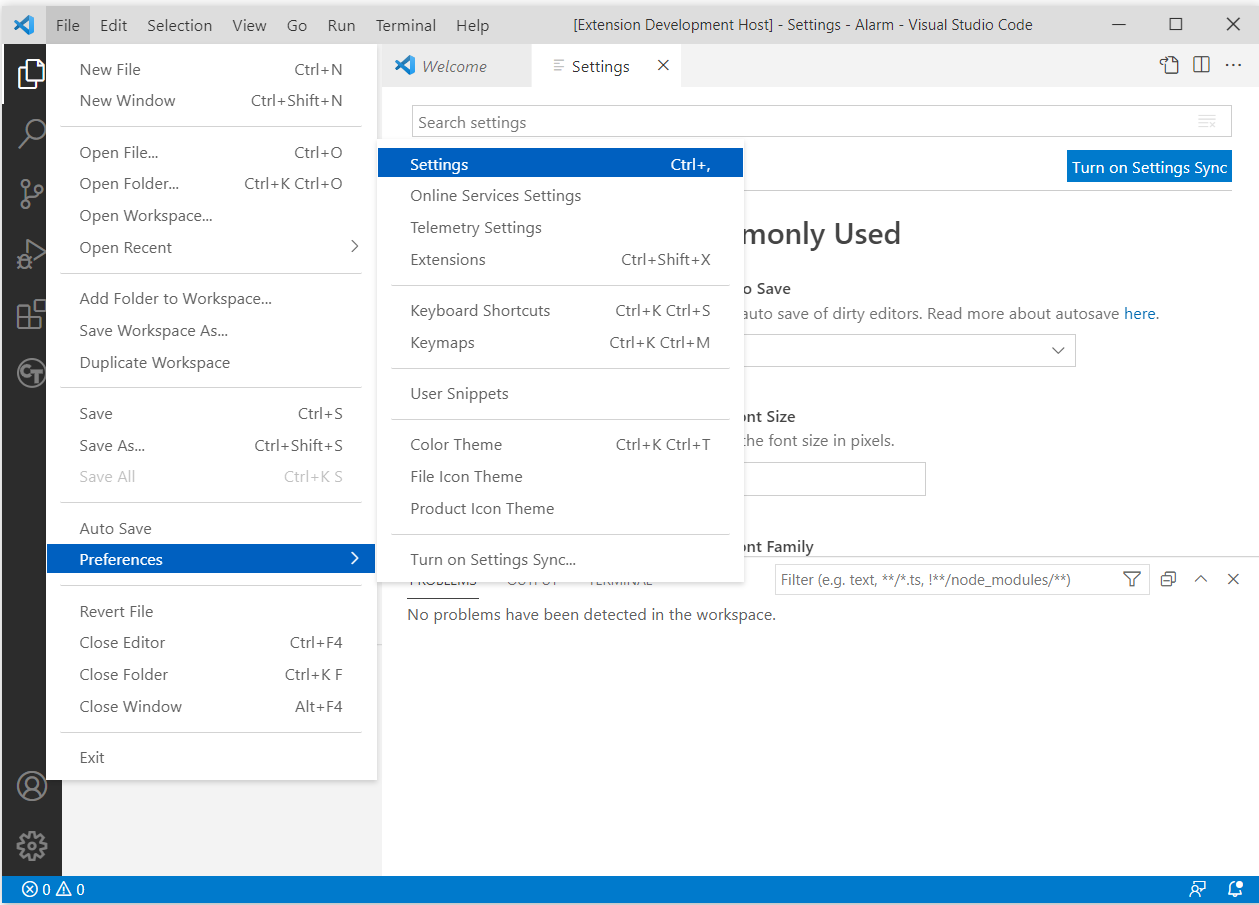
\includegraphics[width=\textwidth]{snapshots/Path to go to settings.png}
  \caption[VDM VSCode Settings]{Path to go to Settings}
  \label{fig:pathVDMSettings}
\end{center}
\end{figure}

\begin{figure}[!hbt]
\begin{center}
  \includegraphics[width=\textwidth]{snapshots/Settings VDM VSCode.PNG}
  \caption[Overture Project Settings]{VDM VSCode Settings}
  \label{fig:VDMSettings}
\end{center}
\end{figure}





\chapter{Editing VDM Models}\label{sec:editVDM}

\section{VDM Dialect Editors}

VDM model files are always ment to be changed in the dialect Editor area. Syntax checking
is carried out continuously as source files are
changed (even before the files are saved). Whenever files are saved, assuming
there are no syntax errors, a full type check of the \emph{entire} VDM model is
performed.
Problems and warnings will be listed in the Problems window as well as
being highlighted directly in the Editor area where the problems have been
identified.


\section{Using Templates}\label{sec:templates}

VSCode templates can be particularly useful when you are new to
writing VDM models. If you press \textit{CTRL+space} after typing the
first few characters of a template name, Overture will offer a
proposal. For example, if you type ''fun'' followed by
\textit{CTRL+space}, the IDE will propose the use of an implicit or
explicit function template as shown in
Figure~\ref{fig:functionTemplate}. The IDE includes several templates:
cases, quantifications, functions (explicit/implicit), operations
(explicit/implicit) and many more. The use of templates makes it much
easier for users to create models, even if they are not deeply
familiar with the VDM syntax.

\begin{figure}
\begin{center}
\includegraphics[width=6in]{snapshots/Explicit function template.png}
\caption{Explicit function template}
\label{fig:functionTemplate}
\end{center}
\end{figure}



\chapter{Interpretation and Debugging in Overture}\label{sec:debug}

This chapter describes how to run and debug a model using the Overture VSCode Extension.

\section{Run and Debug Launch Configurations}\label{sec:launchmodes}

To execute or debug a VDM model, you must first create a launch
configuration\index{debug configuration}. To do this, follow the instructions below. 


\begin{enumerate}
    \item Right click in the EXPLORER (red square) to display the different available options
    \item Click on ‘Add VDM Run Configuration’ (highlighted in blue)
    \item  Write your input entry point module ('DEFAULT' in our case)
    \item Write your input entry point function or operation ('Run(e1)' in our case with ‘Run’ the function and ‘e1’ the argument)
\end{enumerate}

Finally, you can see in Figure~\ref{fig:userguide:new.jsonFile} the newly created configuration file.


\begin{figure}[htp]
\begin{center}
  \includegraphics[width=380px]{snapshots/Add VDM Run Configuration.PNG}
  \caption{Adding VDM Run Configuration}
  \label{fig:userguide:launchconfig}
\end{center}
\end{figure}

\begin{figure}[htp]
\begin{center}
  \includegraphics[width=400px]{snapshots/Input entry point module.PNG}
  \caption{Input Entry Point Module}
  \label{fig:userguide:launchconfigRToptions}
\end{center}
\end{figure}


\begin{figure}[htp]
\begin{center}
  \includegraphics[width=460px]{snapshots/Input entry point function.PNG}
  \caption{Input Entry Point Function/Operation}
  \label{fig:userguide:launchconfigSpecialoptions}
\end{center}
\end{figure}



\begin{figure}[htp]
\begin{center}
  \includegraphics[width=460px]{snapshots/New .json file with the VDM Run Configuration.png}
  \caption{New .json file with the configuration}
  \label{fig:userguide:new.jsonFile}
\end{center}
\end{figure}

\cleardoublepage
On the other hand, you can also create a launch.json file by default without entering module or function, see Figure~\ref{fig:userguide:DefaultLaunch.json}.

\begin{figure}[htp]
\begin{center}
  \includegraphics[width=460px]{snapshots/Creating a launch.json by default.png}
  \caption{Creating a launch.json file by default}
  \label{fig:userguide:DefaultLaunch.json}
\end{center}
\end{figure}

\begin{enumerate}
    \item Click on 'create a launch.json file'
    \item Then a window appear, thus select an environment ('VDM Debug' if you want to configure a VDM project)
\end{enumerate}

\newpage
In addition, you have the possibility to add other configurations. You just have to go in the Run view and follow the instructions below.

\begin{figure}[htp]
\begin{center}
  \includegraphics[width=460px]{snapshots/Add Configuration.PNG}
  \caption{Adding an other VDM Run Configuration}
  \label{fig:userguide:AddingOtherConfig}
\end{center}
\end{figure}

\begin{enumerate}
    \item Click on the button ‘Add Configuration...’ (bottom right corner), or on the arrow facing downwards and press ‘Add Configuration...’
    \item Select the configuration that you want to add to your project (‘VDM Debug: Entry Point (VDM-SL)’ in our case, highlighted in grey)
\end{enumerate}

\clearpage
\section{The Run View}

The Run view\index{debug perspective} contains all the views
commonly needed for debugging in VDM. Breakpoints can easily be set in the
model by clicking in the left margin of the Editor view at the chosen
line. Then a red dot will appear next to the number of the selected line. When the debugger reaches the location of a breakpoint and stops, you can
inspect the values of different identifiers and step through the VDM model
line by line.\index{perspective!debug}

The Run view is illustrated in Figure~\ref{fig:userguide:DebuggingVDM}.

\begin{figure}[htp]
\begin{center}
  \includegraphics[width=460px]{snapshots/Run and Debug a .json file.PNG}
  \caption[Run view]{Run and Debug a .json File}
  \label{fig:userguide:DebuggingVDM}
\end{center}
\end{figure}



\begin{enumerate}
    \item Click on the button ‘Run and Debug’(Ctrl+Shift+D) to have access to the Run view (red square)
    \item Select with the arrow facing downwards which configuration you want to launch
    \item Finally, click on the \includegraphics[width=0.025\textwidth]{snapshots/Icon Start Debugging.png}(‘Start Debugging’ (F5)) to run and debug the configuration selected
    \item If you want to display the debug console, click in the yellow square and click on ‘Debug Console’
\end{enumerate}


\chapter{Collecting Test Coverage Information}\label{sec:testcoverage}

When a VDM model is being interpreted, it is possible to automatically collect
test coverage information. Test coverage measurements help you to see how well a
given test suite\index{Test Coverage!Test suite} exercises your VDM model.

Before generating coverage, there is one prerequisite, you have to run and debug a VDM model. You can see more details about running and debugging a VDM model in the Figure~\ref{fig:userguide:DebuggingVDM}.

In order to enable the collection of test coverage data, right click on a file in the Explorer and select the \emph{Generate coverage} option (See Figure~\ref{fig:userguide:pathTestCoverage}). After
launching this coverage, a new file with a \texttt{.covtbl} extension will be created. This file is written into a project subfolder named
\texttt{.generated/coverage <date and time>}. 


\begin{figure}[htp]
\begin{center}
  \includegraphics[width=160px]{snapshots/Path to generate coverage.png}
  \caption[Path to generate coverage]{Path to Generate Coverage}
  \label{fig:userguide:pathTestCoverage}
\end{center}
\end{figure}

Thus, all highlighted text represents the code used for running the test. We can see that in our case the operation 'NumberOfExperts' is not used in our test because this part of the code is not highlighted in blue (see Figure~\ref{fig:userguide:testCoverage}). 

\begin{figure}[htp]
\begin{center}
  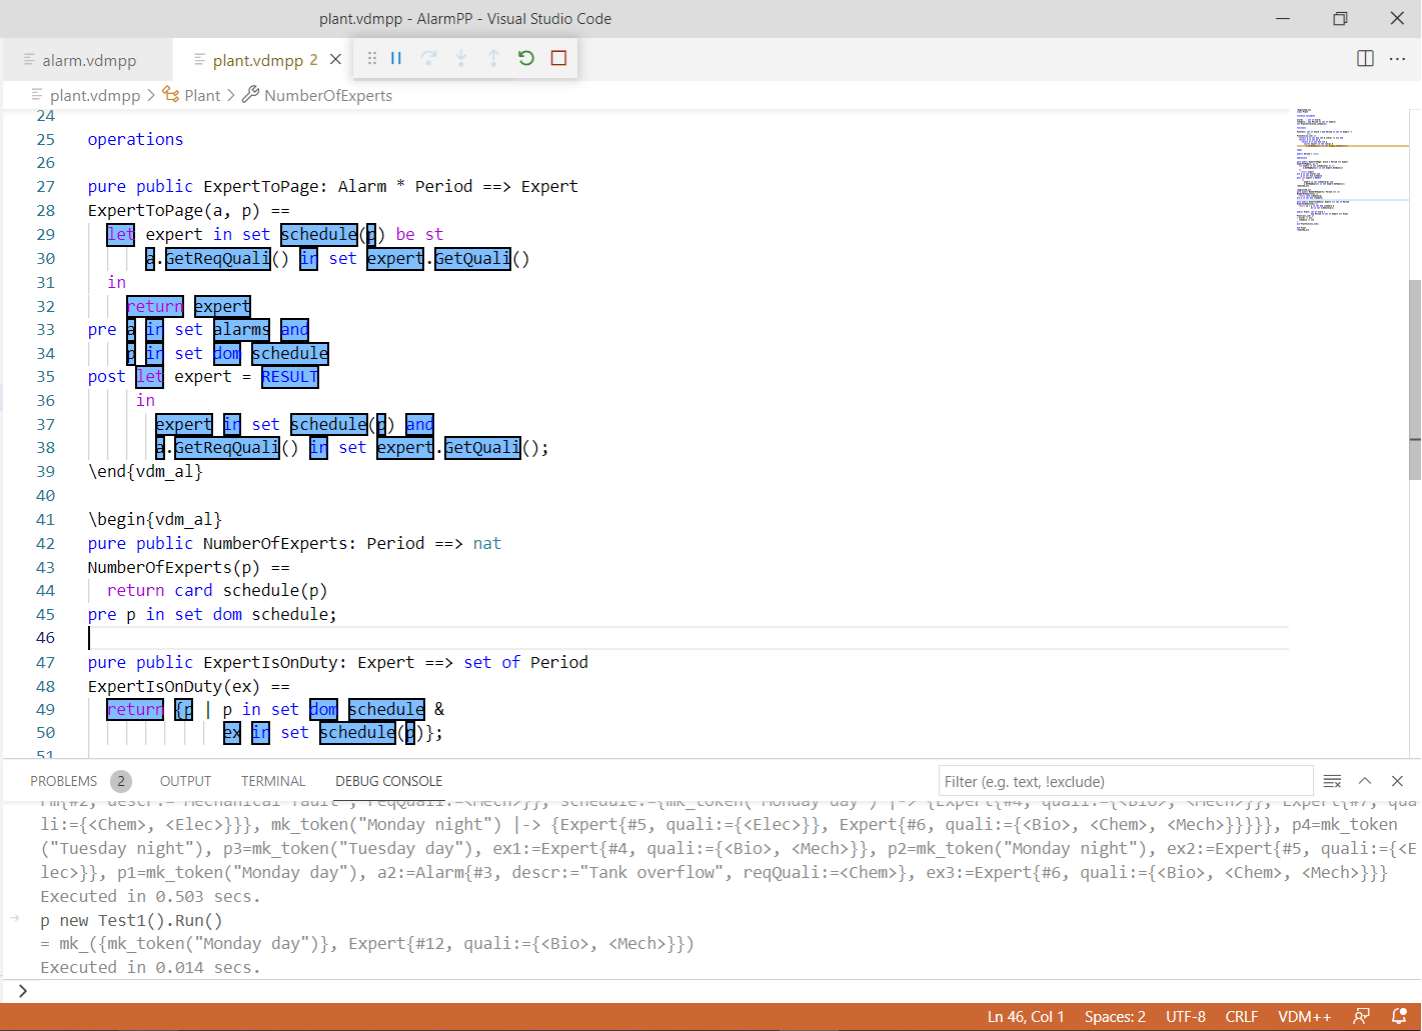
\includegraphics[width=460px]{snapshots/Test coverage.png}
  \caption[Test coverage]{Test Coverage}
  \label{fig:userguide:testCoverage}
\end{center}
\end{figure}

\chapter{Pretty Printing to \LaTeX}\label{sec:prettyprint}

%Include \texttt{overture.tex} which among other things makes use of the
%\texttt{times.cls} and \texttt{listings.cls} style classes. This enables
%the use of the standard \texttt{lstlisting} environment for type setting
%source text and display it in a fixed width font where all VDM keywords
%are typeset in bold.

It is possible to use literate programming/specification \cite{Johnson96} with
Overture just as you can with VDMTools. To take advantage of this,
you need to use the \LaTeX\ text processing system with
plain VDM models mixed with textual documentation.  The VDM model parts must be
enclosed within ``\verb+\begin{vdm_al}+'' and ``\verb+\end{vdm_al}+''. The
text-parts outside these specification blocks are ignored by the VDM parser,
though note that each source file must start with a recognizable \LaTeX\
construct: a \verb+\documentclass, \section, \subsection+ or a \LaTeX\ comment.


To use this functionality, you just have to right click on a file and select 'Translate to LaTeX'. Thus, a new file with a \texttt{.tex} extension will be created. This file is written into a project subfolder named \texttt{.generated/latex <date and time>}.



\chapter{Managing Proof Obligations}\label{sec:POmanagement}

In all VDM dialects, Overture can identify places where run-time errors
\emph{could} potentially occur if the model was to be executed. The analysis of
these areas can be considered
as a complement to the static type checking that is performed automatically.
Type checking accepts specifications that are \emph{possibly} correct, but
we also want to know the places where the specification could possibly fail.

Unfortunately, it is not always possible to statically check if such
potential problems will \emph{actually} occur at run-time error or not. So Overture
creates \emph{Proof Obligations}\index{proof obligation} for all the places
where run-time errors \emph{could} occur. Each proof obligation (PO)
is formulated as a predicate that must hold at a particular place in the VDM
model if it is error-free, and so it may have particular context information
associated with it. POs can be considered as
constraints that will guarantee the internal integrity of a VDM model if they
are all met. In the long term, it will be possible to prove these constraints
with a proof component in Overture, but this is not yet available.

POs can be divided into different categories\index{proof obligation!categories}
depending upon their nature. The full list of categories can be found in
Appendix~\ref{app:POcategories} along with a short description for
each of them.

The proof obligation generator is invoked either on a VDM project (and
then POs for all the VDM model files will be generated) or for one
selected VDM file. Right-click the file in the Explorer and
then select \emph{Run Proof Obligation Generation}. Overture will change into a special
\emph{Proof Obligations} view\index{proof
  obligation!perspective} as shown in
Figure~\ref{fig:POView}.\index{perspective!proof obligation} Once you have
generated POs for a VDM project for the first time, they will automatically be
re-generated whenever the project is rebuilt as long as you stay in the
\emph{Proof Obligations} view.

\begin{figure}[htbp]
\begin{center}
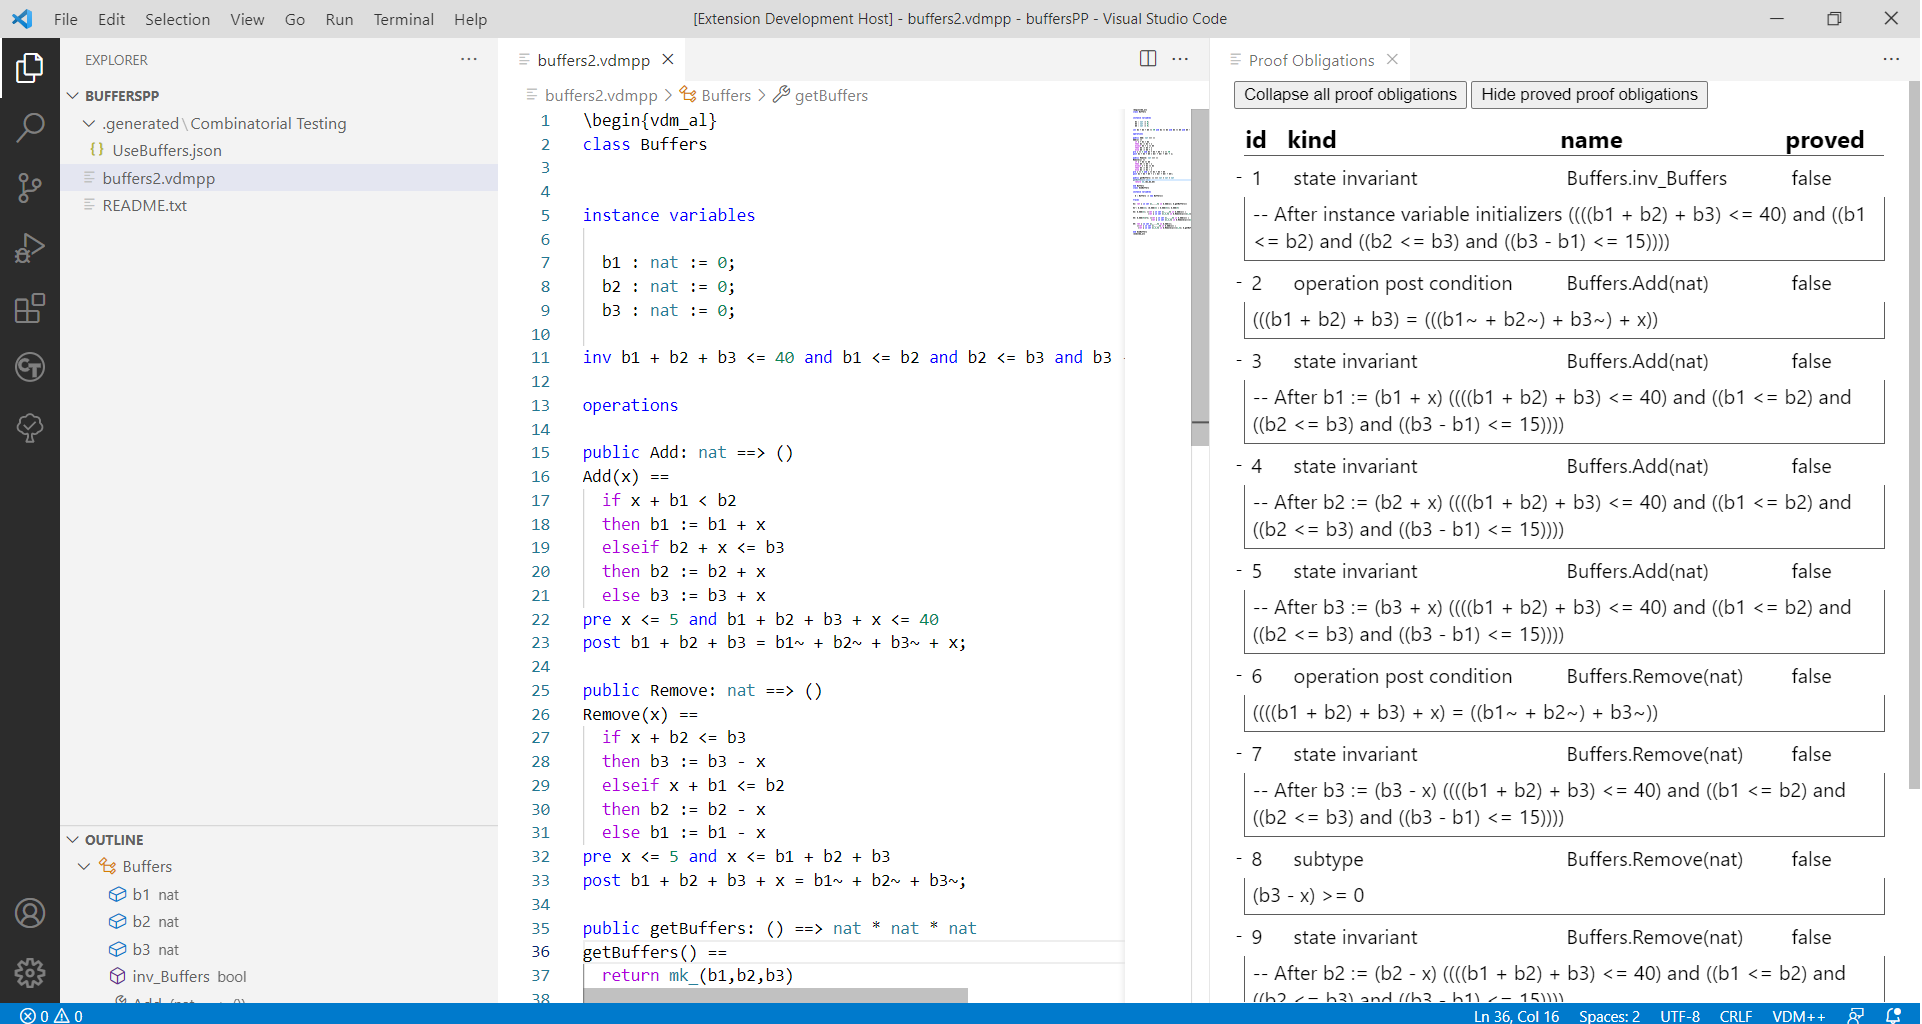
\includegraphics[width=\textwidth]{snapshots/Proof obligation perspective.png}
\caption{The Proof Obligation view\label{fig:POView}}
\end{center}
\end{figure}

Note that in the \emph{Proof Obligation View} view, each proof
obligation has four components:
\begin{itemize}
\item A unique number in the list shown;
\item The proof obligation category (type);
\item The name of the definition in which the proof obligation is located; and
\item The proved proof obligations (true or false).

\blankline

Moreover, you are able to expand or collapse all proof obligations with the buttons 'Expand all proff obligations' and 'Collapse all proof obligations'. And you can also display or hide proved proof obligations with the buttons 'Display proved proof obligations' and 'Hide proved proof obligations'.
%; and
%\item A status field indicating whether the proof obligation is
%  trivially correct or would have to be proved by a proof engine.
\end{itemize}

%At the top of the \emph{Proof Obligation Explorer} the \emph{Filter proved} button
%allows you to filter away all the proof obligations that are trivially
%correct.\index{filter proved}

\chapter{Combinatorial Testing}\label{sec:testing}

In order to better automate the testing process, a notion of
test \emph{traces} has been introduced into VDM++ (and subsequently VDM-SL and VDM-RT)\footnote{Note that this is
only available for VDM-SL and VDM-RT models if the VDM-10 language version has been selected.}.
Traces are effectively regular expressions that can be expanded to a collection of test
cases. Each test case comprises a sequence of operation
calls. If a user defines a trace it is possible to make use of a
special \emph{Combinatorial Testing} perspective to automatically
expand the trace and execute all of the resulting test
cases. Subsequently, the results from the tests can be inspected
and erroneous test cases easily found. You can then fix
problems and re-run the trace to check they are fixed.

\section{Using the Combinatorial Testing GUI}

The syntax for trace definitions is defined in the VDM-10 Language
Manual \cite{Larsen&10b}.\index{traces}
If you have created a {\textbf\texttt{traces}} entry for a module or class it
can be executed via the \emph{Combinatorial Testing}
view\index{combinatorial testing}, see
Figure~\ref{fig:tracesalarm}.\index{perspective!combinatorial testing}

Different icons are used to indicate the verdict in a test
case. These are:
\begin{description}
\item[\hspace{-1.8mm}
\raisebox{-0.8mm}{\includegraphics[width=0.02\textwidth]{snapshots/Icon grey dot.png}}:]
  This icon is used to indicate that the test case has not yet been
  executed.
\index{icon!not yet executed}
\item[\hspace{-1.8mm}
\raisebox{-0.8mm}{\includegraphics[width=0.02\textwidth]{snapshots/Icon green dot.png}}:]
  This icon is used to indicate that the test case has a pass
  verdict.\index{icon!pass verdict}
\item[\hspace{-1.8mm}
\raisebox{-0.8mm}{\includegraphics[width=0.02\textwidth]{snapshots/Icon blue dot.png}}:]
  This icon is used to indicate that the test case has an inconclusive
  verdict.\index{icon!inconclusive verdict}
\item[\hspace{-1.8mm}
\raisebox{-0.8mm}{\includegraphics[width=0.02\textwidth]{snapshots/Icon red dot.png}}:]
  This icon is used to indicate that the test case has a fail
  verdict.\index{icon!fail verdict}
\end{description}


In the CT view, you can right-click on any individual
test case, and then send it to the interpreter for execution ('Send test to interpreter'). This is particularly useful for
failed test cases since the interpreter allows you to step through the
evaluation to the place where it is failing. You can inspect the exact
circumstances of the failure, including the values of the different
variables in scope.

\begin{figure}[htbp]
\begin{center}
\includegraphics[width=6.5in]{snapshots/Combinatorial testing.PNG}
\caption{Using Combinatorial Testing\label{fig:tracesalarm}}
\end{center}
\end{figure}

\newpage
\begin{enumerate}
    \item Click on the button ‘Combinatorial Testing’ to have access to the Combinatorial testing view (red square)
    \item Click on the button ‘Generate test outline’
\end{enumerate}


\begin{figure}[htbp]
\begin{center}
\includegraphics[width=6.5in]{snapshots/Launch of the combinatorial tests.PNG}
\caption{Launch of Combinatorial Tests\label{fig:SendToInterpreter}}
\end{center}
\end{figure}

\newpage
\begin{enumerate}
    \item  Click on the button \includegraphics[width=0.03\textwidth]{snapshots/Icon Execute All Tests.png} (‘Execute All Tests’) to launch all the combinatorial tests. Or if you want to launch only one combinatorial test, you can click on \includegraphics[width=0.025\textwidth]{snapshots/Icon Start Debugging.png}  (‘Full Evaluation’).\\
    If you want to add filtering options, click on the button  \includegraphics[width=0.03\textwidth]{snapshots/Icon Set Filter Options.png}  (‘Set Filter Options’) and a window will appear (red square). Now you have the possibility to reduce the number of tests generated depending on the operation name or/and the variable name ('Trace Reduction Type'), to display the traces with a particular value in their seed ('Trace Filtering Seed'), to limit the number of executed tests ('Subset Limitation(\%)'), to reset all the filters changed previously (‘Reset’) or just confirm your changes (‘OK’).
    
    If you want to filter the combinatorial tests in function of their result, you can click on \includegraphics[width=0.03\textwidth]{snapshots/Icon CT Filtering.png} ('Show selected tests') and select one or many options between : 'Passed', 'Failed', 'Inconclusive' and 'Filtered'.
    
    You can also rebuild trace outline with the button  \includegraphics[width=0.03\textwidth]{snapshots/Icon Rebuild Trace Outline.png}  (‘Rebuild Trace Outline’), or collapse all tests with the button  \includegraphics[width=0.03\textwidth]{snapshots/Icon Collapse All.png}  (‘Collapse All’).\\
    Finally, in each test, you have the possibility to filter evaluation with the button \includegraphics[width=0.03\textwidth]{snapshots/Icon Filtered Evaluation.png}  (‘Filtered Evaluation’), to restart the generation of tests with the button  \includegraphics[width=0.03\textwidth]{snapshots/Icon Rebuild Trace Outline.png}  (‘Generate Tests’), or to go to the trace \includegraphics[width=0.03\textwidth]{snapshots/Icon Go To Trace.png}   (‘Go to trace’).
\end{enumerate}
%
% Automatic Code Generation chapter
%

\chapter{Automatic Generation of Code}\label{sec:codegen}

It is possible to generate Java code\index{code generation} for a
large subset of VDM-SL and VDM++ models. In addition to Java, a C++
code generator is currently being developed, but this work is in its
early stages of development, and it is not included with releases of
Overture yet. For comparison, code generation of VDM-SL and VDM++
specifications to both Java and C++ is a feature that is available in
VDMTools~\cite{Java2VDMMan,CGMan,CGManPP}. The sections below focus
solely on the Java code generator available in Overture.

\section{Use of the Java Code Generator}
\label{sec:javacg_use}

\begin{figure}[htbp]
\begin{center}
\includegraphics[width=10cm]{screenDumps/javacg_menu}
\caption{Launching the Java code generator.\label{fig:javacg_menu}}
\end{center}
\end{figure}

\begin{figure}[htbp]
\begin{center}
\includegraphics[width=\linewidth]{screenDumps/javacg_output}
\caption{The status of code generating the \texttt{AlarmPP} example.\label{fig:javacg_output}}
\end{center}
\end{figure}

The Java code generator can be launched via the context menu as shown
in Figure~\ref{fig:javacg_menu}. Alternatively, this can be done by
highlighting the project in the VDM explorer and typing one of the
shortcuts associated to this plugin.\\

\noindent The Java code generator operates in two different modes:

\begin{itemize}

\item \emph{Regular mode:} In this mode the Java code generator
  produces an Eclipse project with all the generated code. Java code
  generation in this mode can also be initiated using the
  \texttt{Ctrl+Alt+C} shortcut.

\item \emph{Launch Configuration mode:}. Is currently limited to
  VDM++. This mode is like regular code generation except that the
  Java code generator also prompts the user for a launch configuration
  as input for the code generation process. Based on this launch
  configuration the Java code generator constructs an entry point (a
  \texttt{main} method really) that serves as an entry point for the
  generated code. Launch configuration based code generation can be
  initiated using the \texttt{Ctrl+Alt+B} shortcut.

\end{itemize}

\noindent Upon completion of the code generation process the status is
output to the console as shown in Figure~\ref{fig:javacg_output}. In
particular this figure shows the status of code generating the
\texttt{AlarmPP} model available in the Overture standard examples. As
indicated by the console output, the generated code is available as an
Eclipse project in the \texttt{<workspace>/<project>/generated/java}
folder.

\section{Configuration of the Java Code Generator}

The Java code generator can be configured via a preference page as
shown in Figure~\ref{fig:javacg_config}. The preference page can be
accessed in the way you would normally access an Eclipse preference
page or via the context menu shown above in
Figure~\ref{fig:javacg_menu}. The Java code generator provides a few
options that allows the user to configure the code generation process
(see Figure~\ref{fig:javacg_config}). The sub-sections below treat
each of these configuration parameters individually, in the order they
appear in the preference page.

\begin{figure}[htbp]
\begin{center}
\includegraphics[width=13cm]{screenDumps/javacg_config}
\caption{Configuration of the Java code generator.\label{fig:javacg_config}}
\end{center}
\end{figure}

\subsection{Disable cloning}

In order to respect the value semantics of VDM the Java code generator
sometime needs to perform deep copying of certain objects that is uses
to represent composite value types (records, tuples, tokens, sets,
sequences and maps). For example, in VDM a record is a value type,
which means that occurrences of the record must be copied when it
appears in the right-hand side of an assignment, it is passed as an
argument or returned as a result. However, Java does not support
composite value types like structs and records, and as a consequence
record types must be represented using classes, which use reference
semantics. This means that an object reference, which is used to
represent a composite value type in the generated Java code must be
deep copied when it appears in the right-hand side of an assignment,
it is passed as an argument or returned as a result. For arbitrarily
complex value types (such as records composed of record or sets of
composed of sets) deep copying may introduce a significant overhead in
the generated code. If the specification subject to code generation
does not truly rely on value semantics the user may wish to disable
deep copying of value types in the generated code in order to remove
this overhead. The user should, however, be aware that disabling of
cloning may lead to code being generated that does not preserve the
semantics of the input specification and in general disabling of
cloning is discouraged. By default cloning is enabled.

\subsection{Generate character sequences as strings}

In VDM a string is a sequence of characters and there is no notion of
a string type. Java in particular works differently since it uses a
separate type to represent a string. The default behaviour of the Java
code generator is to code generate sequences of characters as strings
and subsequently do the necessary conversion between between strings
and sequences in the generated code. Another possibility is to treat a
string literal for what it truly is, namely a sequence of characters,
and thereby avoid any conversion between strings and sequences. In
order to do that, i.e.\ \textit{not} generating character sequences as
strings, the corresponding option must be unchecked.

\subsection{Generate concurrency mechanisms}

If the user does not rely on the concurrency mechanisms of VDM++ and
does not want to include support for them in the generated code the
corresponding option in the preference page must be unchecked. By
default the behaviour of the Java code generator is to not include
support for the concurrency mechanisms of VDM++ in the generated code.

\subsection{Generate Java Modeling Language (JML) annotations}

When a VDM model is code generated to Java all the contract-based
elements of the model, i.e.\ the pre conditions, post conditions and
invariants, are ignored by default. This feature does, however,
provide limited support for translation of the contract-based elements
of a VDM-SL model. When the corresponding option is checked the
contract-based elements are translated to JML~\cite{Burdy&05}
annotations which are added on top of the generated Java code as
source code comments. This allows the system properties, expressed in
terms of pre conditions, post conditions and invariants, to be checked
against the generated code.\\

\noindent Please note that this feature is still experimental and only
has limited support for checking of named type invariants.

\subsection{Choose output package}

The Java code generator allows the output package of the generated
code to be specified. If the user does not specify a package, the code
generator outputs the generated Java code to a package with the same
name as the VDM project. If the name of the project is not a valid
java package, then the generated code is output to the default Java
package.

\subsection{Skip classes during the code generation process}

It may not always make sense to code generate every class in a
project. Classes that can often be skipped include classes that act as
execution entry points or classes that are used to load input for the
specification. Classes that the user wants to skip can be specified in
the text box in the Java code generator preference page by separating
the class names by a semicolon. As an example, \texttt{World;Env}
makes the code generator skip code generation of the \texttt{World}
and \texttt{Env} classes, while generating code for any other
class. For convenience the output of the Java code generator will also
inform the user about what classes are being skipped.

\section{Limitations of the Java Code Generator}

In case the Java code generator encounters a construct that it cannot
code generate it will report it as unsupported to the user and the
user can then try to rewrite that part of the specification using
other (supported) constructs. Reporting of unsupported constructs is
done via the console output and using editor markers. In order to
demonstrate this, Figure~\ref{fig:javacg_unsupported} shows the
console output of the Java code generator when it encounters a type
bind, which is an example of an unsupported language construct. Note
the small marker appearing in the editor in order to point out where
use of the construct appears. By hovering the corresponding marker the
user will see the reason for why the construct is unsupported. For the
type bind example in Figure~\ref{fig:javacg_unsupported} the reason
is:\\

\noindent \texttt{Following constructs are not supported:\\ \{b |
b:(bool * bool)\} (ASetCompSetExp) at 6:11. Reason:\\Generation of a
set comprehension is only supported for\\multiple set binds. Got:
b:(bool * bool)}\\

\begin{figure}[htbp]
\begin{center}
\includegraphics[width=\linewidth]{screenDumps/javacg_unsupported}
\caption{Reporting of unsupported constructs in the
console.\label{fig:javacg_unsupported}}
\end{center}
\end{figure}

The user will get similar messages and markers for other unsupported
VDM constructs. To summarise, the Java code generator currently does
not support code generation of multiple inheritance and neither does
it support traces, type bind, invariant checks and pre and post
conditions. Furthermore, let expressions appearing on the right-hand
side of an assignment will also be reported as unsupported. Code
generation of patterns is also fairly limited and includes the
identifier, ignore, record and tuple patterns as well as the
character, boolean, integer, nil, quote, real and string match values.

\section{The Code Generation Runtime Library}

The generated code relies on a runtime library used to represent some
of the types available in VDM (tokens, tuples etc.) as well as
collections and support for some of the complex operators such as
sequence modifications. For simplicity every Eclipse project generated
by the Java code generator contains the runtime library. More
specifically, there is a copy of the runtime library containing only
the binaries (\texttt{lib/codegen-runtime.jar}) as well as a version
of the runtime library that has the source code attached
(\texttt{lib/codegen-runtime-sources.jar}). The runtime library is
imported by every code generated class using the Java import statement
\texttt{\textbf{import} org.overture.codegen.runtime.*;} and in order
to compile the generated Java code the runtime library must be visible
to the Java compiler.

Similar to VDMTools the runtime library also provides implementation
for subset of the functionality available in the standard libraries:
The runtime library provides a full implementation of the
\texttt{MATH} library, support for conversion of values into character
sequences as provided by the \texttt{VDMUtil}, and finally
functionality to write to the console as available in the \texttt{IO}
library.







\appendix
\newpage

\bibliographystyle{nnewalpha}

\bibliography{bib/UserGuide,bib/dan}
\addcontentsline{toc}{section}{\protect\numberline{}{References}}



\newpage
\chapter{Internal Errors}\label{app:internalerrors}

This appendix gives a list of the internal errors in Overture
and the circumstances under which each internal error can be expected.
Most of these errors should \emph{never} be seen, so if they appear
please report the occurrence via the Overture bug reporting utility
(\url{https://github.com/overturetool/overture/issues/new}).

\input{MESSAGES_Internal}

\newpage
\chapter{Lexical Errors}\label{app:lexerr}

When a VDM model is parsed, the first phase is to gather the single
characters into tokens that can be used in the further
processing. This is called a lexical analysis and errors in this area
can be as follows:

\input{MESSAGES_Lexical}

\newpage
\chapter{Syntax Errors}\label{app:synerr}

If the syntax of the file you have provided does not meet the
syntax rules for the VDM dialect you wish to use, syntax errors will be
reported. These can be as follows:

\input{MESSAGES_Syntax}

\newpage
\chapter{Type Errors and Warnings}\label{app:typeerr}

If the syntax rules are satisfied, it is still possible to get
errors from the type checker. The errors can be as
follows:

\input{MESSAGES_TypeChecking}

Warnings from the type checker include:

\input{MESSAGES_Warnings}

\newpage
\chapter{Run-Time Errors}\label{app:runtimeerr}

When using the interpreter/debugger it is possible to get run-time
errors, even if there are no type checking errors. The possible errors
are as follows:

\input{MESSAGES_Runtime}

\newpage
\chapter{Categories of Proof Obligations}\label{app:POcategories}

This appendix provides a list of the different proof obligation
categories generated by Overture, and an explanation of the
circumstances under which each category can be expected.

\input{podescriptions}


\newpage
\chapter{Mapping Rules between VDM++/VDM-RT and UML Models} \label{chap:umlrules}

\begin{formationRule}
\label{rule:transformationRuleClasses}
VDM classes are mapped as the UML meta-class \texttt{Class}
\end{formationRule}

\begin{formationRule}
\label{rule:transformationRuleVisibility}
The visibility of VDM instance variables, values, functions and operations are mapped as a \textit{subset} of the UML enumeration \texttt{VisibilityKind} comprising \kw{public}, \kw{private} and \kw{protected}.
\end{formationRule}

\begin{formationRule}
\label{rule:transformationRuleStatic}
VDM \kw{static} is mapped as the \texttt{isStatic} property of the UML meta-class \texttt{Class}, \texttt{Property} or \texttt{Operation} respectively.
\end{formationRule}

\begin{formationRule}
\label{rule:Datatypes}
Data type definitions are mapped as the UML meta-class \texttt{Class} and are referenced, and thus nested, through the meta-attribute \texttt{nestedClassifier} of the owning class.
Notice that this rule is not specified or implemented.
%, hence Figure \ref{fig:dataTypeNestedClass} is not generated by the tool made as part of this thesis.
\end{formationRule}

\begin{formationRule}
\label{rule:InstanceVarsAndValuesAsAssoc}
Instance variable and value definitions are mapped as the UML meta-class \texttt{Association}, if:
\begin{description}
\item \textbf{\ref{rule:InstanceVarsAndValuesAsAssoc} a:} The type is an \textit{object reference type}, or
\item \textbf{\ref{rule:InstanceVarsAndValuesAsAssoc} b:} The type is \textit{not} a basic \textit{data type} \cite[p64,71]{Fitzgerald&05}.
\end{description}%
\end{formationRule}

\begin{formationRule}
\label{rule:InstanceVarsAndValuesAsProp}
Instance variable and value definitions are mapped as the UML meta-class \texttt{Property}, if the type is a \textit{basic data type} \cite[p71]{Fitzgerald&05}. Instance variables and values are distinguished by the meta-attribute \texttt{isReadOnly}. Notice: rule 
%\ref{rule:transformationRuleConstraint} and 
\ref{rule:transformationRuleMap} is an exception to this rule.
\begin{center}
\begin{tabular}{|l|c|}
\hline
VDM concept & \texttt{Property::isReadOnly}\\
\hline
 Instance variables & \texttt{false}\\
 Values & \texttt{true}\\
\hline
\end{tabular}
\captionof{table}{The meta-attribute \texttt{isReadOnly} distinguishes instance variables and values}
\label{tab:instanceVariablesValuesTransRule}
\end{center}
\end{formationRule}

\begin{formationRule}
\label{rule:InstanceVarsAndValuesInitialValue}
The initial value of instance variables and values definitions are mapped as the property \texttt{default} of the UML meta-class \texttt{Property}.
\end{formationRule}

\begin{formationRule}
\label{rule:InstanceVarsAndValuesOptional}
The VDM optional type is mapped to the properties \texttt{lower = 0} and \texttt{upper = 1} of the UML meta-class.
\end{formationRule}
%
% \begin{formationRule}
%% \label{rule:transformationRuleConstraint}
%% A union type is mapped as the meta-class \texttt{Association} between the owning class and the types specified in the union type. The resulting associations are decorated with a textual constraint \texttt{\{xor\}}. The constraint is an instance of the meta-class \texttt{Constraint}.
%% Notice, that if a member of a union type is a \textit{basic type}, it is mapped as a separate UML class. This is an exception to rule \ref{rule:InstanceVarsAndValuesAsProp}
%% \end{formationRule}

%% \begin{formationRule}
%% \label{rule:transformationRuleProductType}
%% A VDM product type maps to:
%% \begin{description}

%% \item \textbf{\ref{rule:transformationRuleProductType} a:} The UML meta-class \texttt{Class} if it is declared as a data type. 
%See figure \ref{fig:PersonAssociationNWithTypeDeclared}.

%% \item \textbf{\ref{rule:transformationRuleProductType} b:} The UML meta-class \texttt{Association} if it is not defined as a type (i.e.\ it is anonymous). 
%See figure \ref{fig:PersonAssociationN} and \ref{fig:productType}.

%% \end{description}
%% Each association-end that represents an entry in the product type is named according to the product type. The types constituting the product type are sorted alphabetically according to the name of the types used in the product type.
%% \end{formationRule}

\begin{formationRule}
\label{rule:transformationRuleSetSeqSeq1}
The VDM constructs \kw{set}, \kw{seq} and \kw{seq1} is mapped as the UML meta-class \texttt{Association} which may be decorated with a textual constraint defined by the meta-attribute \texttt{isOrdered\footnotemark} in addition to a multiplicity at both ends. Table \ref{tab:staticSetSeqSeq1TransRule} shows how the above-mentioned VDM constructs are mapped.\\

\begin{center}
\begin{tabular}{|l|c|c|c|}
\hline
VDM construct & Ordered & Target class Multiplicity  \\
\hline
 \kw{set} & \texttt{false}  & \texttt{0..*}\\
 \kw{seq} & \texttt{true} & \texttt{0..*}\\
 \kw{seq1} & \texttt{true} & \texttt{1..*}\\
\hline
\end{tabular}

\captionof{table}{Transformation rules for VDM constructs modeling collections}

\label{tab:staticSetSeqSeq1TransRule}
\end{center}
\end{formationRule}

\begin{formationRule}
\label{rule:transformationRuleMap}
The VDM constructs \kw{map} and \kw{inmap} are mapped as the UML meta-class \texttt{Association} with a qualifier. The domain is specified by the qualifier, which is located at the source class. The range is specified by the target class. 
Notice, that if the range is specified by a \textit{basic type} it is mapped as a separate class. This is an exception to rule \ref{rule:InstanceVarsAndValuesAsProp}.

\begin{center}
\begin{tabular}{|l|c|c|}
\hline
\multirow{2}{*}{VDM construct} & Qualifier end & Target class end \\
 & \texttt{isUnique} & \texttt{isUnique} \\
\hline
 \kw{map} & \texttt{false} & \texttt{true}\\
 \kw{inmap} &\texttt{true} & \texttt{true}\\
\hline
\end{tabular}
\captionof{table}{Transformation rules for VDM constructs modeling relationships between two sets.} 
%See figure \ref{fig:UniqueMapImap}}
\label{tab:qualifiedAssocTransRule}
\end{center}
\end{formationRule}

\begin{formationRule}
\label{rule:transformationRuleThread}
A VDM class with a \kw{thread} compartment is mapped as the UML meta-class \texttt{Class} with the meta-attribute \texttt{isActive} set to \texttt{true}.
\end{formationRule}

\begin{formationRule}
\label{rule:transformationRuleGeneralization}
A VDM class with the keyword \kw{is subclass of} followed by class-names is mapped as the UML meta-class \texttt{Generalization}, with the attributes \texttt{general} and \texttt{specific} referencing the superclass and subclass, respectively.
More than one subclass results in more than one instance of \texttt{Generalization}.
\end{formationRule}

\begin{formationRule}
\label{rule:transformationRuleAbstract}
A VDM class with the keyword \kw{is subclass responsibility} as a function or operation body is mapped as the UML meta-class \texttt{Class} with the meta-attribute \texttt{isAbstract} set to \texttt{true}.
\end{formationRule}

\begin{formationRule}
\label{rule:transformationRuleTemplate}
A VDM generic class maps to the UML meta-class \texttt{Class} with the attribute \texttt{templateSignature} referencing a set of \texttt{TemplateParameter} having the name property set to the name of the parameter.
\end{formationRule}

\begin{formationRule}
\label{rule:transformationRuleOperationFunction}
A VDM operation and function are mapped to the UML meta-class \texttt{Operation} where the property \texttt{isQuery} determine whether the \texttt{Operation} represents a VDM function or operation:
\begin{itemize}
    \item \kw{true} for a function.
	\item \kw{false} for a operation.
\end{itemize}
\\
The return type of a function and operation is mapped collectively as the property \texttt{type} and the multiplicity\footnotemark of the \texttt{Operation} meta-class.
The parameters of the operation or function is mapped to the UML meta-class \texttt{Parameter} represented as the property \texttt{ownedParameters} of the \texttt{Operation} meta-class.\\
The name and type of a VDM parameter are mapped to the property \texttt{name}, \texttt{type} and the multiplicity\footnotemark[\thefootnote] of the \texttt{Parameter} meta-class.
\end{formationRule}

\newpage
\chapter{Using VDM Values in Java}\label{cha:VDMvalues}

Integration between Overture and Java code can be established, either by writing native libraries in Java that can be called from VDM, or by giving a Java program overall control of a VDM model by making calls to that model as a user interacts with a GUI.

In both cases, internal VDM values have to be handled by Java -– either because they are passed as arguments to a Java library, and returned as results to VDM, or because they are returned from a VDM model evalution to a controlling Java program.

This appendix describes the internal class hierarchy used by Overture to represent internal VDM model values, and describes how a Java program can convert these to Java values (\kw{int}, \kw{long}, \kw{String} etc.) as well as creating internal values for returning to the VDM model (e.g.\ as the return value of library methods).

\section{The Value Class Hierarchy}

All internal VDM values in Overture are held by instances of the \texttt{Value}
class with the fully qualified name,
\texttt{org.overture.interpreter.values.Value}. The \texttt{Value} class itself
is abstract, but subclasses can be instantiated to represent any VDM value,
such as a ``\kw{seq of char}'', ``\kw{nat1}'” or a value of an arbitrarily
complex type. The hierarchy is shown in Figure~\ref{fig:gui:JavaVDMhierarchy}.

Generally, the name of the \texttt{Value} subclass for a VDM type is on the form \texttt{<\textit{name}>Value}, for example \texttt{BooleanValue} or \texttt{SeqValue}.
 
The following sections describe how to obtain Java values from a \texttt{Value} object, and how to create \texttt{Value} objects from basic Java values (or iteratively from other values).

\section{Primitive Values}

Most primitive VDM types have subclasses with simple constructors that take a Java primitive type as an argument:

\begin{lstlisting}[language=JAVA]
public BooleanValue(boolean value)
public CharacterValue(char value)
public RealValue(double value) throws Exception
public RationalValue(double value) throws Exception
public IntegerValue(long value)
public NaturalValue(long value) throws Exception
public NaturalOneValue(long value) throws Exception
public QuoteValue(String value)
public NilValue()
\end{lstlisting}

The constructors that throw exceptions are the ones for which some Java value does not match the VDM type concerned. For example, a \texttt{RealValue} or \texttt{RationalValue} cannot take the Java values \texttt{Double.NaN} or \texttt{Double.POSITIVE\_INFINITY} as a constructor argument. Similarly, \texttt{NaturalValue} and \texttt{NaturalOneValue} cannot take a negative long as an argument.

\begin{figure}[h]
\begin{center}
  \includegraphics[width=2.5in]{screenDumps/ValueHierarchy}
  \caption[labelInTOC]{Java Value Hierarchy}
  \label{fig:gui:JavaVDMhierarchy}
\end{center}
\end{figure}

Note that a \texttt{QuoteValue} is constructed with a string. This is simply the string value that would appear between angle brackets in VDM, for example \texttt{<FAIL>} would be constructed with the Java string \texttt{"FAIL"}.

To convert a VDM value into a Java value, the \texttt{Value} class provides a number of conversion methods, each of which returns the corresponding Java primitive value, or throws an exception if the conversion cannot be made for the VDM type concerned:

\begin{lstlisting}[language=JAVA]
public boolean boolValue(Context ctxt) throws ValueException
public char charValue(Context ctxt) throws ValueException
public double realValue(Context ctxt) throws ValueException
public double ratValue(Context ctxt) throws ValueException
public long intValue(Context ctxt) throws ValueException
public long natValue(Context ctxt) throws ValueException
public long nat1Value(Context ctxt) throws ValueException
public String quoteValue(Context ctxt) throws ValueException
\end{lstlisting}

Note that all of these conversion functions take a \texttt{Context} parameter as argument and potentially throw a \texttt{ValueException}. The \texttt{Context} parameter is used internally by Overture and represents the call stack during the evaluation of an expression. This parameter can be set to null when using these methods in Java code outside Overture. A \texttt{ValueException} is thrown if the VDM value cannot be converted into the Java type requested. For example, calling \texttt{booleanValue} on a \texttt{RealValue} object will raise a \texttt{ValueException} with the message text \texttt{"Can't get bool value of real"}.

\section{Sets, Sequences and Maps}

VDM allows primitive types to be built into more complex aggregations and collections, and these can also be converted to and from Java types, though the process is a little more involved. Three classes are provided to assist with this conversion: \texttt{ValueSet}, \texttt{ValueList} and \texttt{ValueMap} (all within the same  \url{org.overture.interpreter.values} package). These classes represent, respectively, a Java \texttt{Set}, \texttt{List} and \texttt{Map} of VDM values:

\begin{lstlisting}[language=JAVA]
public class ValueSet extends Vector<Value>
public class ValueList extends Vector<Value>
public class ValueMap extends LinkedHashMap<Value, Value>
\end{lstlisting}

Note that the \texttt{ValueSet} class is actually based on a Java \texttt{Vector}, not a Java \texttt{Set} type, though the class does have set semantics (no duplicates). This is an implementation detail and allows Overture to permute set orderings in certain circumstances.

These three classes have obvious constructors, and allow \texttt{Value}s (or collections of them) to be added to the collection subsequently, using standard Java collection methods:

\begin{lstlisting}[language=JAVA]
public ValueSet()
public ValueSet(int size)
public ValueSet(ValueSet from)
public ValueSet(Value v)

public ValueList()
public ValueList(ValueList from)
public ValueList(Value v)
public ValueList(int size)

public ValueMap()
public ValueMap(ValueMap from)
public ValueMap(Value k, Value v)
\end{lstlisting}

Using these three helper classes, it is now possible to create VDM set, sequence and map values, using constructors of the \texttt{SetValue}, \texttt{SeqValue} and \texttt{MapValue} classes:

\begin{lstlisting}[language=JAVA]
public SetValue()
public SetValue(ValueSet values)

public SeqValue()
public SeqValue(ValueList values)
public SeqValue(String s)

public MapValue()
public MapValue(ValueMap values)
\end{lstlisting}

Note that there is a special constructor for \texttt{SeqValue} that takes a Java string. This creates a VDM ``\kw{seq of char}'', but without the need to create a \texttt{ValueList} with \texttt{CharacterValue}s.

If the \texttt{ValueList} (or another) collection passed to these constructors contains a mixture of VDM types -– i.e.\ a mixture of VDM \texttt{Value} subclasses, such as a \texttt{BooleanValue} and a \texttt{NaturalOneValue} -– then the type of the constructed VDM value is the union of the various types passed, in this example ``\kw{seq of (bool} \texttt{$\mid$} \kw{nat1)}''. If this VDM type is not compatible with the use of a corresponding value in the VDM model a dynamic type exception occurs when the value is processed by the model.

Lastly, as before, to get the primitive Java values of a VDM collection, the following methods are provided:

\begin{lstlisting}[language=JAVA]
public ValueList seqValue(Context ctxt) throws ValueException
public String stringValue(Context ctxt) throws ValueException
public ValueSet setValue(Context ctxt) throws ValueException
public ValueMap mapValue(Context ctxt) throws ValueException
\end{lstlisting}

Note that, as with the \texttt{SeqValue} constructor, there is a special method to return a Java String from a ``\kw{seq of char}'' \texttt{SeqValue}, rather than a \texttt{ValueList} of \texttt{CharacterValue}s. As before, if the \texttt{Value} being used is not a sequence, set or map, then these methods will throw a \texttt{ValueException}.

\section{Other Types}

The sections above describe how to create or deconstruct simple VDM values in Java as well as simple collections of these. The remainder of this section describes the unusual cases, for more sophisticated types.

\subsection{Function values}

Overture has an internal \texttt{FunctionValue} class used for holding values of functions (e.g.\ the value of a ``{\textbf\ttfamily lambda}'' expression or the value of a function defined within a module). But as far as Java is concerned, these values are opaque -– there is no equivalent Java construct, and the only way to evaluate a VDM function is to let Overture perform that evaluation. Similarly, Java cannot construct a \texttt{FunctionValue}.

The only operation that Java can reasonably perform with a \texttt{FunctionValue} is to create a composite function (eg. ``\texttt{f1 comp f2}'' in VDM) or a function iteration (e.g.\ ``\texttt{f ** 3}'' in VDM) using existing \texttt{FunctionValue}s. In order to do this, there are two subclasses of \texttt{FunctionValue}, called \texttt{CompFunctionValue} and \texttt{IterFunctionValue}, the constructors for which are as follows:

\begin{lstlisting}[language=JAVA]
public CompFunctionValue(FunctionValue f1, FunctionValue f2)
public IterFunctionValue(FunctionValue function, long count)
\end{lstlisting}

These both create new \texttt{FunctionValue}s, which when evaluated by Overture act as the composition and iteration of the arguments, respectively.

There is a method for obtaining a \texttt{FunctionValue} from a \texttt{Value}, but note that this is not an internal Java value (unlike other \texttt{Value} methods, like \texttt{realValue}). It is used as a more convenient way of casting the \texttt{Value} to a \texttt{FunctionValue}.

\begin{lstlisting}[language=JAVA]
public FunctionValue functionValue(Context ctxt)
\end{lstlisting}

\subsection{Object Values}

When VDM++ and VDM-RT create new objects using the ``\kw{new}'' operator, the resulting values are held as \texttt{ObjectValue}s in Overture. These are complex types that involve function and operation definitions for the object as well as any type, value, sync, thread or traces sections defined. Therefore \texttt{ObjectValue}s are really opaque to Java and cannot be used directly.

Like for \texttt{FunctionValue}, the \texttt{ObjectValue} class has a method for converting a \texttt{Value} into an \texttt{ObjectValue}:

\begin{lstlisting}[language=JAVA]
public ObjectValue objectValue(Context ctxt)
\end{lstlisting}

\subsection{Record Values}

A VDM record is just a collection of typed field values. A \texttt{RecordValue} can be obtained from a \texttt{Value} using the following method, which returns a \texttt{RecordValue} rather than some other Java representation:

\begin{lstlisting}[language=JAVA]
public RecordValue recordValue(Context ctxt)
\end{lstlisting}

To get individual field values from a \texttt{RecordValue}, two more Java helper types have to be introduced, called \texttt{FieldMap} and \texttt{FieldValue}. A \texttt{FieldValue} has the following constructor, and represents a record field:

\begin{lstlisting}[language=JAVA]
public FieldValue(String name, Value value, boolean comparable)
\end{lstlisting}

The \texttt{comparable} argument indicates whether this field is used in the value comparison between record values. A field declared with ``\texttt{-}'' in VDM would have a false argument, but normally this argument would be true, and the value must match the record type being used. \texttt{FieldValue}s are added to a \texttt{FieldMap}, which is just a Java \texttt{List} of \texttt{FieldValue}s.

So given a \texttt{RecordValue}, its \texttt{FieldMap} can be obtained from a public final field in the object, called \texttt{fieldMap}\footnote{Really this ought to have a get method.}, and from there, individual \texttt{FieldValue}s can be accessed -– e.g.\ \texttt{fieldMap.get(0).name} and \texttt{fieldmap.get(0).value}.

To create a \texttt{RecordValue}, the record type is obtained from the \texttt{RemoteInterpreter}:

\begin{lstlisting}[language=JAVA]
type = remoteInterpreter.getInterpreter().findType(typename)
\end{lstlisting}

The type is then passed to the \texttt{RecordValue} constructor, along with a \texttt{FieldMap} or a \texttt{ValueList} (of the fields in order).

\begin{lstlisting}[language=JAVA]
public RecordValue(RecordType type,
		   ValueList values, 
		   Context ctxt)
public RecordValue(RecordType type, 
		   FieldMap mapvalues, 
		   Context ctxt)
\end{lstlisting}

The \texttt{Context} parameter is needed to allow records with invariants to check the invariant before the value is constructed. Note that currently, record types with an invariant cannot be constructed in Java. The \texttt{Context} parameter can be passed as null from Java.

The caller is responsible for passing field values that match their expected type. If they do not match, Overture throws a dynamic type exception for subsequent evaluations.

\subsection{Token Values}

Token values are simply wrappers for normal VDM values, reflecting the way they are created in VDM, like \texttt{mk\_token("hello")}, which would be a wrapper for a ``{\textbf\ttfamily seq of char}''. There is no special way of getting a \texttt{TokenValue} from a \texttt{Value}, other than casting it. Having casted the \texttt{Value}, the wrapped value can be obtained from the public final \texttt{Value} field called ``\texttt{value}''.

Constructing a \texttt{TokenValue} is just a matter of passing the \texttt{Value} required:

\begin{lstlisting}[language=JAVA]
public TokenValue(Value exp)
\end{lstlisting}

\subsection{Tuple Values}

A \texttt{TupleValue} in Overture is a wrapper for a \texttt{ValueList}. The following method and constructor can be used like one would expect:

\begin{lstlisting}[language=JAVA]
public TupleValue(ValueList argvals)
public ValueList tupleValue(Context ctxt)
\end{lstlisting}

\subsection{Invariant Values}

A VDM type can be given a name and an invariant, e.g.\ when wrapping a primitive type without an invariant. Overture has a separate \texttt{Value} subclass for values of such types that simply combine the primitive \texttt{Value} with a \texttt{FunctionValue} for the invariant. However, as with \texttt{RecordValue}s (which can also have invariants), it is not currently possible to create \texttt{InvariantValue}s in Java for types that have an invariant.

For types without an invariant, the constructor is as follows:

\begin{lstlisting}[language=JAVA]
public InvariantValue(NamedType type, Value value, Context ctxt)
\end{lstlisting}

The \texttt{NamedType} is obtained in a similar way to the \texttt{RecordType} above, using the \texttt{Remote\-Interpreter}. Note that the caller is responsible for passing a \texttt{Value} that matches the expected type. If they do not match, Overture will throw a dynamic type exception for subsequent evaluations.

\subsection{Void Values}

Operations which do not return a value in VDM (i.e.\ \texttt{==> ()}) return an instance of \texttt{VoidValue} in Java. The constructor has no arguments.

\newpage%\section{Index}
\phantomsection
\label{sec:index}
\addcontentsline{toc}{chapter}{Index}
\printindex
%\addcontentsline{toc}{section}{\protect\numberline{}{Index}}



\end{document}
